\documentclass[10pt,aspectratio=169]{beamer}

% --- Thème et Couleurs ---
\usetheme{Madrid}
\usecolortheme{whale}
\definecolor{myblue}{RGB}{0, 90, 160}
\setbeamercolor{structure}{fg=myblue}
\setbeamercolor{title}{fg=white, bg=myblue}
\setbeamercolor{frametitle}{fg=white, bg=myblue}

% --- Paquets indispensables ---
\usepackage[utf8]{inputenc}
\usepackage[T1]{fontenc}
\usepackage[french]{babel}
\usepackage{graphicx}
\usepackage{listings}
\usepackage{xcolor}
\usepackage{booktabs}
\usepackage{tikz}

% --- Configuration des listings (pour le code) ---
\definecolor{codebg}{RGB}{248,248,248}
\lstset{
	backgroundcolor=\color{codebg},
	basicstyle=\ttfamily\tiny,
	keywordstyle=\color{myblue}\bfseries,
	frame=single,
	rulecolor=\color{gray},
	breaklines=true,
	showstringspaces=false
}

% --- Informations du titre ---
\title[Sujet 2 : Robot Aspirateur]{Planification en Intelligence Artificielle \\ Sujet 2 : Robot Aspirateur en PDDL et Fast Downward}
\author[Master 1 Informatique]{KIMBUNGU SIMEON Gédéon \and LABEM KAPINGA Ketsia \and KALEMBU MASIRIKA Constantin \and TANDU KIKALANGA Nathan \and LUNGA KABITA Supreme \and MUJINGA MATAMBA PLAMEDI}
\institute[UNIKIN]{Université de Kinshasa \\ Faculté des Sciences et Technologies \\ Doctorant Patrick MANYA}
\date{Année Académique 2025--2026}

\begin{document}
	
	% --- Diapositive 1 : Page de garde ---
	\begin{frame}
		\titlepage
	\end{frame}
	
	% --- Diapositive 2 : Le Problème ---
	% --- Diapositive 2 : Le Problème ---
	\begin{frame}{Le Problème}
		\begin{columns}
			\column{0.6\textwidth}
			
			\textbf{Définition :} Un robot aspirateur est un appareil électroménager autonome conçu pour nettoyer les sols (poussières, miettes, poils) sans intervention humaine directe.
			
			\vspace{0.4cm}
			
			\textbf{Le défi :} Nettoyer un logement de 4 pièces.
			
			\vspace{0.3cm}
			\begin{itemize}
				\item Le robot ne peut pas se téléporter.
				\item Il doit se déplacer entre les pièces via des passages.
				\item Il ne peut nettoyer que là où il se trouve.
			\end{itemize}
			
			\vspace{0.3cm}
			\textbf{Objectif :} Trouver un ordre de visite et de nettoyage pour que toutes les pièces soient propres à la fin.
			
			\column{0.4\textwidth}
			\centering
			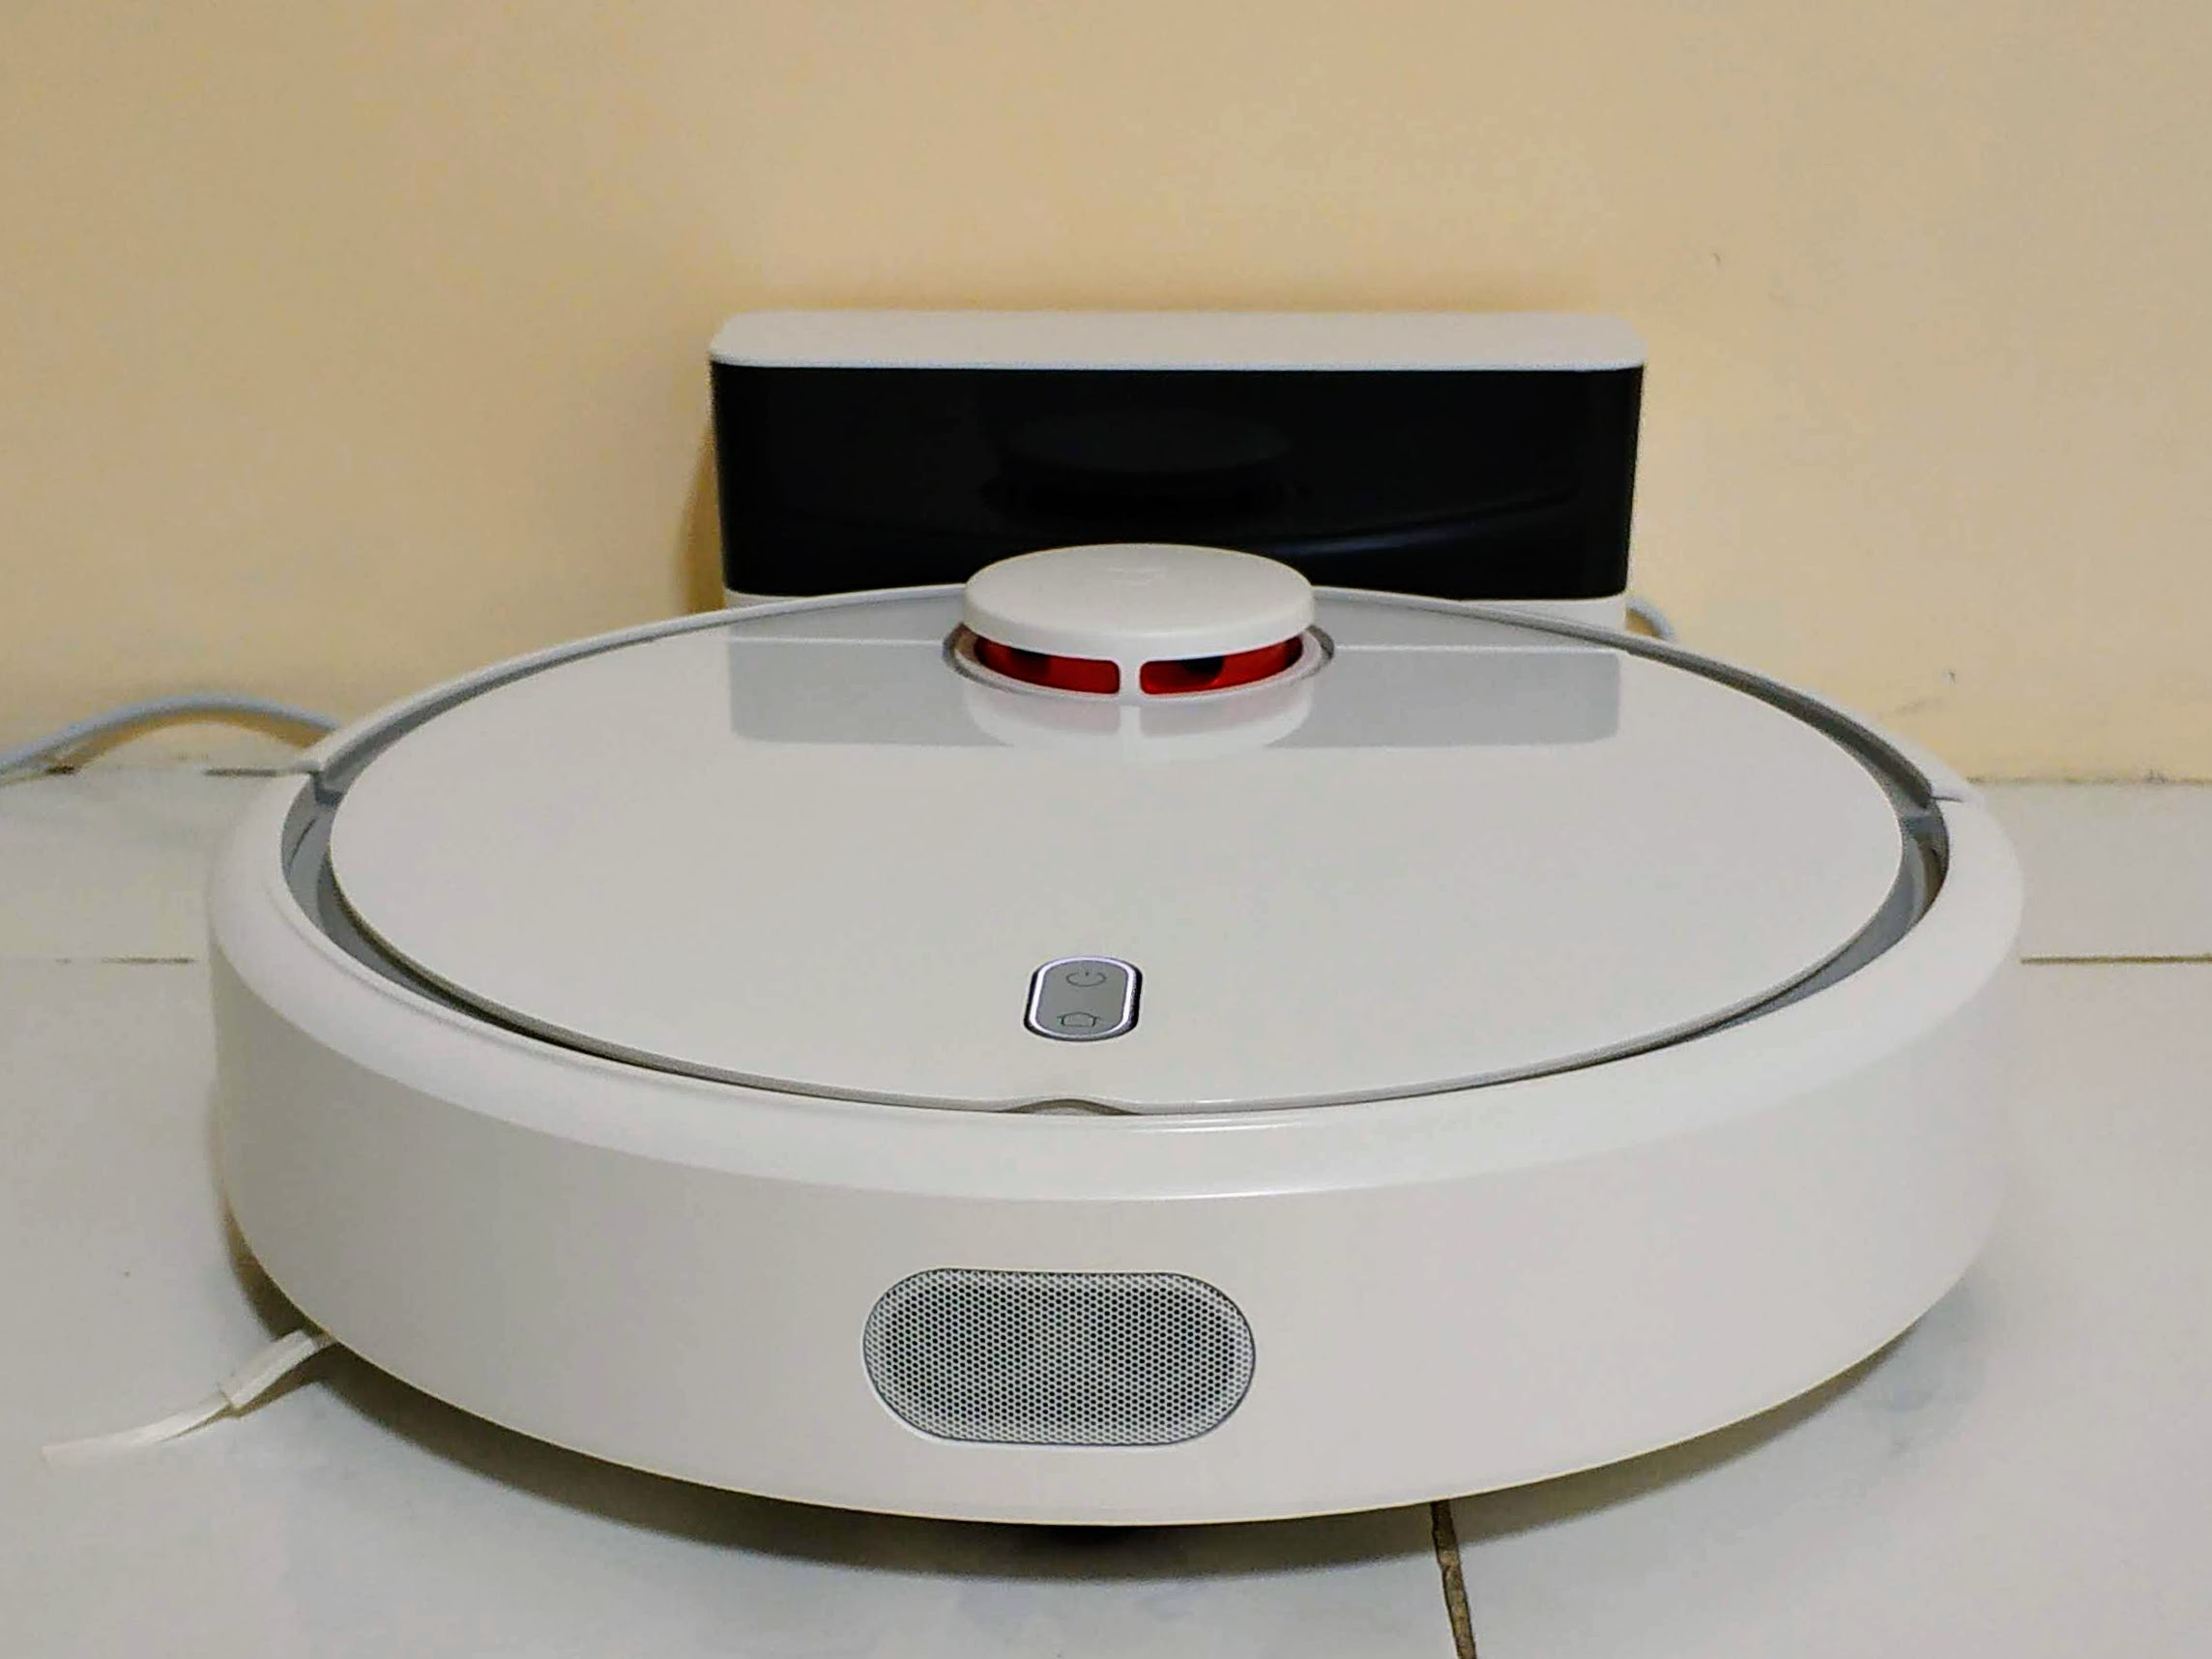
\includegraphics[width=0.9\textwidth]{images/Xiaomi_robot_vacuum.jpeg}
			
			\vspace{0.1cm}
			{\tiny Source : Par Nowforever — Travail personnel, CC BY-SA 4.0, Wikimedia Commons.}
		\end{columns}
	\end{frame}
	
	% --- Diapositive 3 : Modélisation du Logement ---
	\begin{frame}{Modélisation du Logement}
		\begin{columns}
			\column{0.65\textwidth}
			\centering
			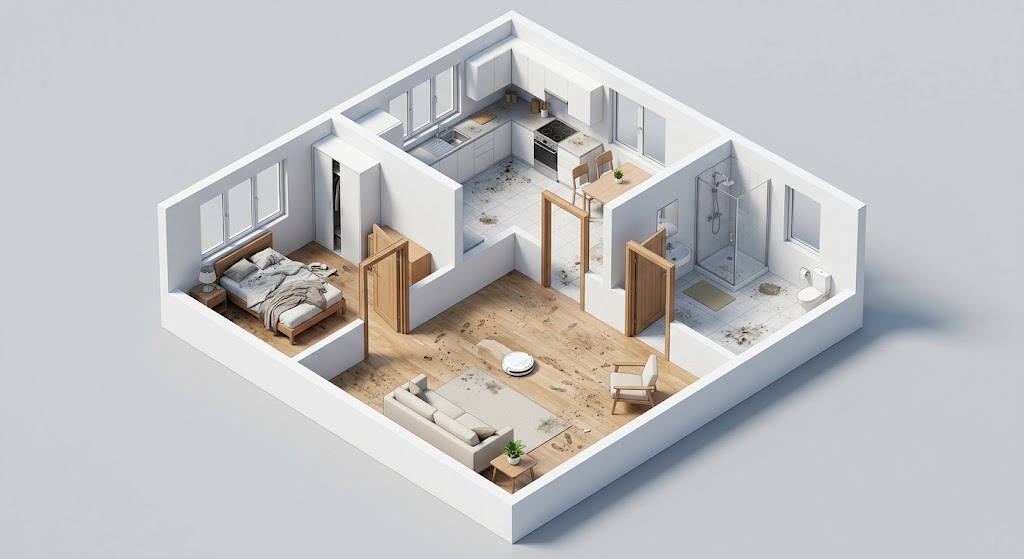
\includegraphics[width=\textwidth]{captures/vue_3D.png}
			\caption{Topologie du logement (Salon = nœud central)}
			
			\column{0.35\textwidth}
			\textbf{Points clés :}
			\begin{itemize}
				\item 4 pièces : Cuisine, Salon, Chambre, SDB.
				\item Toutes reliées au salon.
				\item Aucune connexion directe entre les pièces périphériques.
			\end{itemize}
		\end{columns}
	\end{frame}
	
	% --- Diapositive 4 : Modélisation PDDL ---
	\begin{frame}{Modélisation PDDL : Les Actions}
		\textbf{Deux actions suffisent pour modéliser le robot :}
		
		\vspace{0.3cm}
		\begin{block}{Action \texttt{move} (Déplacement)}
			\textbf{Préconditions :} Robot dans la pièce de départ + Passage existant. \\
			\textbf{Effets :} Robot dans la pièce d'arrivée (et plus dans celle de départ).
		\end{block}
		
		\begin{block}{Action \texttt{clean} (Nettoyage)}
			\textbf{Préconditions :} Robot dans la pièce + Pièce sale. \\
			\textbf{Effets :} Pièce propre (et plus sale).
		\end{block}
	\end{frame}
	
	% --- Diapositive 5 : Fast Downward ---
	\begin{frame}[fragile]{Le Planificateur : Fast Downward}
		\textbf{Un planificateur en C++ basé sur STRIPS/PDDL.}
		
		\vspace{0.5cm}
		\textbf{Commande utilisée :}
		\begin{lstlisting}[language=bash]
			python3 ~/downward/fast-downward.py \
			domain.pddl problem.pddl \
			--search "astar(blind())"
		\end{lstlisting}
		
		\vspace{0.3cm}
		\begin{itemize}
			\item \textbf{Algorithme :} A* avec heuristique aveugle (garantit un plan optimal).
			\item \textbf{Résultat :} Plan de 9 actions en quelques millisecondes.
		\end{itemize}
	\end{frame}
	
	% --- Diapositive 6 : Résultat (Le Plan) ---
	% --- Diapositive 6 : Résultat (Le Plan) ---
	\begin{frame}[fragile]{Résultat : Le Plan Optimal (9 actions)}
		\begin{columns}
			% Colonne de gauche : Le plan textuel
			\column{0.42\textwidth}
			\textbf{Le plan généré :}
			\begin{lstlisting}[basicstyle=\tiny\ttfamily, frame=single]
				1. move  r1 salon chambre
				2. clean r1 chambre
				3. move  r1 chambre salon
				4. move  r1 salon cuisine
				5. clean r1 cuisine
				6. move  r1 cuisine salon
				7. clean r1 salon
				8. move  r1 salon sdb
				9. clean r1 sdb
			\end{lstlisting}
			
			\vspace{-0.2cm}
			\textbf{Analyse :}
			\begin{itemize}\itemsep0em
				\item Passage central obligatoire (Salon).
				\item Nettoyage du salon à l'étape 7.
			\end{itemize}
			
			% Colonne de droite : Le graphe du parcours
			\column{0.58\textwidth}
			\centering
			\begin{tikzpicture}[
				scale=0.75, transform shape,
				room/.style={draw, rectangle, rounded corners=3pt, minimum width=2.2cm, minimum height=0.9cm, fill=blue!10, thick},
				arrow/.style={->, >=stealth, thick, blue!50!black}
				]
				% Définition couleur si non définie globalement
				\definecolor{myblue}{RGB}{0, 102, 204}
				
				% Placement des pièces
				\node[room] (cuisine) at (0, 2.4) {Cuisine};
				\node[room] (chambre) at (-2.6, 0) {Chambre};
				\node[room] (salon)   at (0, 0)   {Salon};
				\node[room] (sdb)     at (2.6, 0)   {SDB};
				
				% Passages physiques (lignes pointillées de fond)
				\draw[gray, dashed, thin] (cuisine) -- (salon);
				\draw[gray, dashed, thin] (chambre) -- (salon);
				\draw[gray, dashed, thin] (salon) -- (sdb);
				
				% 1. Salon -> Chambre
				\draw[arrow, bend right=25] (salon) to node[above, font=\scriptsize] {1} (chambre);
				% 2. Chambre (nettoyage)
				\node[font=\tiny\bfseries, text=red] at (-2.6, -0.7) {2. clean};
				% 3. Chambre -> Salon
				\draw[arrow, bend right=25] (chambre) to node[below, font=\scriptsize] {3} (salon);
				
				% 4. Salon -> Cuisine
				\draw[arrow, bend left=25] (salon) to node[left, font=\scriptsize] {4} (cuisine);
				% 5. Cuisine (nettoyage)
				\node[font=\tiny\bfseries, text=red] at (0, 3.3) {5. clean};
				% 6. Cuisine -> Salon
				\draw[arrow, bend left=25] (cuisine) to node[right, font=\scriptsize] {6} (salon);
				
				% 7. Salon (nettoyage)
				\node[font=\tiny\bfseries, text=red] at (0, -0.6) {7. clean};
				
				% 8. Salon -> SDB
				\draw[arrow, bend left=25] (salon) to node[above, font=\scriptsize] {8} (sdb);
				% 9. SDB (nettoyage)
				\node[font=\tiny\bfseries, text=red] at (2.6, -0.7) {9. clean};
				
			\end{tikzpicture}
		\end{columns}
	\end{frame}
	
	% --- Diapositive 7 : Simulateur (Le Wow Effect) ---
	\begin{frame}{Vérification : Simulateur Web 3D}
		\begin{columns}
			\column{0.6\textwidth}
			\centering
			% Remplacer par votre capture d'écran
			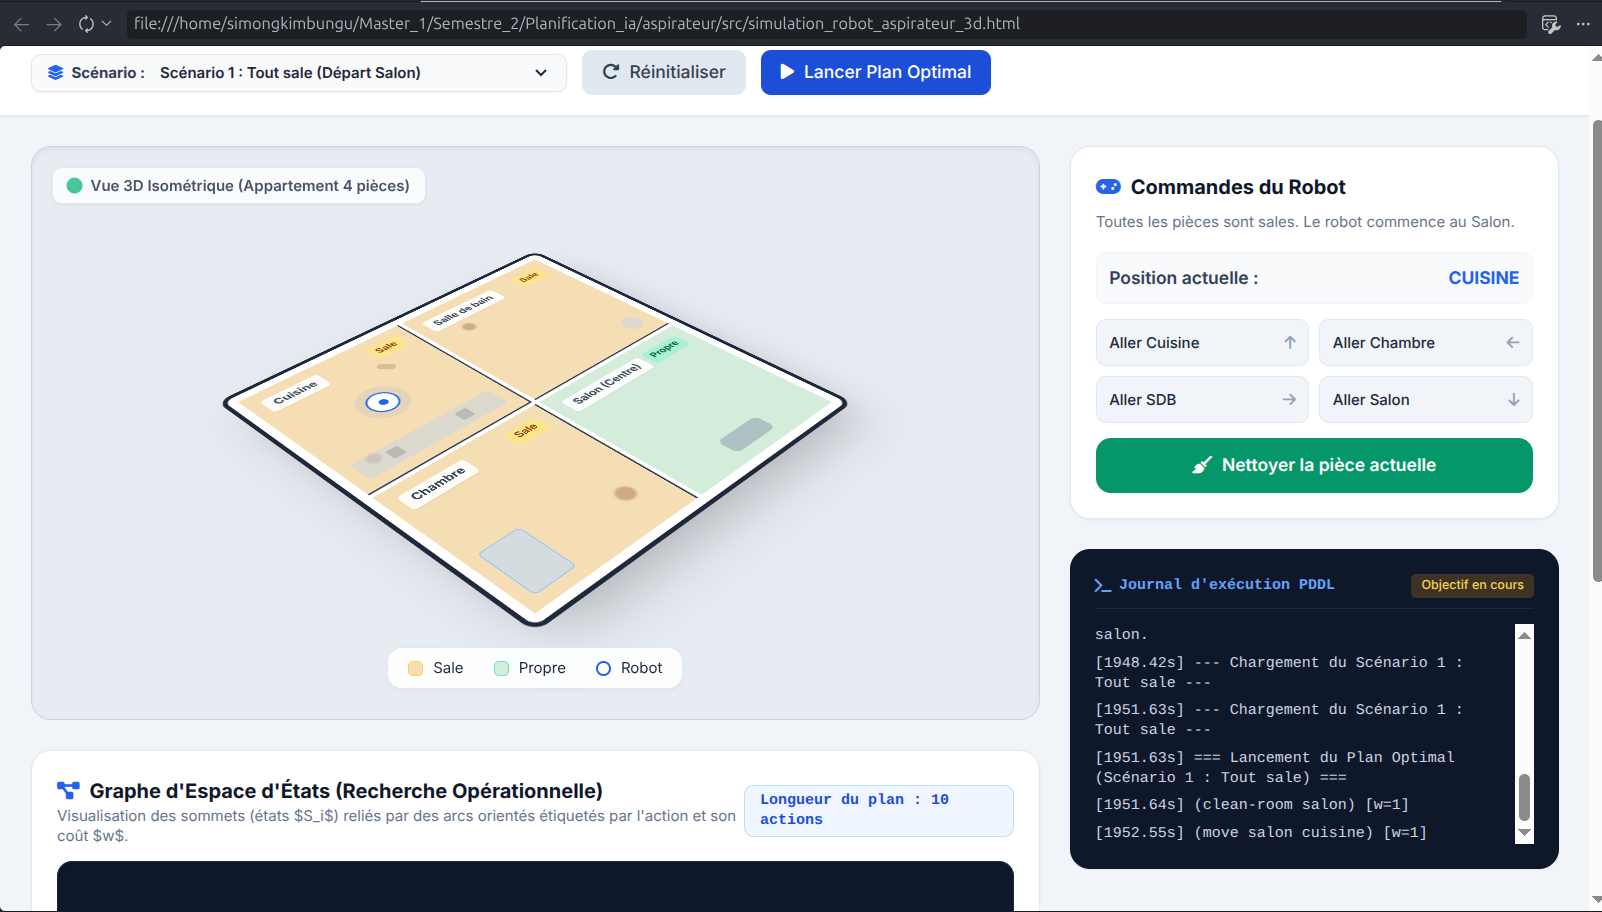
\includegraphics[width=\textwidth]{captures/simulateur_3d.png}
			
			\column{0.4\textwidth}
			\textbf{Validation :}
			\begin{itemize}
				\item Rejoue le plan action par action.
				\item Vérifie les préconditions à chaque étape.
				\item Interface 3D interactive.
			\end{itemize}
			
			\vspace{0.3cm}
			\textit{"C'est la preuve visuelle que notre modèle fonctionne."}
		\end{columns}
	\end{frame}
	
	% --- Diapositive 8 : Scénarios Alternatifs ---
	\begin{frame}[fragile]{Scénarios Alternatifs}
		\begin{columns}
			\column{0.5\textwidth}
			\textbf{Scénario 2 : Cuisine déjà propre}
			\begin{itemize}
				\item Le plan passe de 9 à 6 actions.
				\item Le robot ne visite pas la cuisine.
				\item \textit{Les préconditions éliminent les branches inutiles.}
			\end{itemize}
			
			\vspace{0.3cm}
			\begin{lstlisting}
				move  r1 salon chambre
				clean r1 chambre
				move  r1 chambre salon
				clean r1 salon
				move  r1 salon sdb
				clean r1 sdb
			\end{lstlisting}
			
			\column{0.5\textwidth}
			\textbf{Scénario 3 : SDB inaccessible}
			\begin{itemize}
				\item Passage `salon-sdb` retiré.
				\item Fast Downward affiche :
			\end{itemize}
			\begin{lstlisting}
				No relaxed solution! 
				Task is provably unsolvable.
			\end{lstlisting}
			\textit{Le modèle respecte la topologie : sans passage, le but est inatteignable.}
		\end{columns}
	\end{frame}
	
	% --- Diapositive 9 : Conclusion ---
	\begin{frame}{Conclusion}
		\begin{columns}
			\column{0.5\textwidth}
			\textbf{Ce que nous avons appris :}
			\begin{itemize}
				\item Formaliser un problème réel en STRIPS/PDDL.
				\item Utiliser un planificateur automatique.
				\item Vérifier un plan avec un simulateur indépendant.
			\end{itemize}
			
			\column{0.5\textwidth}
			\textbf{Pistes d'amélioration :}
			\begin{itemize}
				\item Ajouter une notion de temps.
				\item Gérer des obstacles dynamiques.
				\item Comparer différentes heuristiques (hmax, lmcut).
			\end{itemize}
		\end{columns}
		
		\vspace{1cm}
		\centering
		\Large \textit{Merci de votre attention !}
	\end{frame}
	
\end{document}